\status{review}
\chapter{Kalman filter}
{\itshape
This Appendix is to illustrate the working principle of a Kalman filter, showing a simple linear problem in 2D. This is taken, with minor adjustments, from my Master Thesis: In situ monitoring of the stopped muon flux at Mu2e. Although during my PhD I did not implement any Kalman filter, this concept is central in MEG II analysis as well as the muEDM upcoming track fitting and in modern particle physics at large.}
\label{ch:Kalman}

\status{review}
\section{The problem}
    Once the pattern recognition algorithms have been executed, a preliminary but rough estimate of the track parameters $\vec{\eta}$ is available. 
    At this point, there are still numerous effects that should be accounted for when trying to optimize track reconstruction. 
    Some of these effects are obvious, like, for example, the non-uniformity of the magnetic field, while others are less so. 
    An example of the latter is the fact that a hit might have an intrinsic symmetry in a specific detector. \\

    \noindent
    Mathematically, a track can be parameterized using a running variable and a vector of parameters. 
    To make an example, quite often in particle physics, the particles move in magnetic fields, following a helicoidal trajectory. 
    In this case the vector $\vec{\eta}$ with the helix parameters and the position along the beam axis $z$ can be used: $F(\vec{\eta};z)$. 
    The fitting procedure then determines the best estimate of the vector $\vec{\eta}$ and the corresponding covariance matrix $V$. 
    The task gets substantially more complicated if the parameters vector depends on the running variable $\vec{\eta}(z)$. 
    This is the case when the traveling particle can lose energy, interact with some material along its path, or when the magnetic field is not uniform. 
    These are common conditions and the effect in terms of variation of the track parameters values can be substantial.
    Fig. \ref{_Kutschke_Kalman_circ} shows one possible simple example \cite{Kutschke}.
    Now the procedure of finding the `optimal' track parameters suddenly implies also that we need to define the position where we want to determine those parameters.
    It is often the case we are interested in determining the value of $\vec{\eta}$ at the target because this is where the physical process takes place. 

    \begin{figure}[h!]
        \centering
        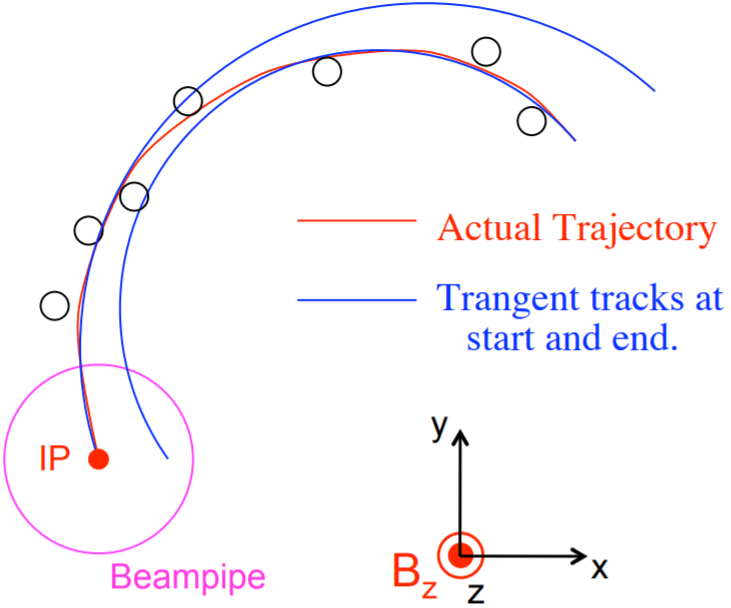
\includegraphics[scale=0.5]{Figures/MEG/Kutschke_Kalman_circ.png}
        \caption[Trajectory with variable parameters]{Pictorial view of the trajectory of a particle traveling along a circular path which has variable parameters \cite{Kutschke}. The two blue circles represent the tangent circles at the beginning and at the end of the track segment: both circles are separately valid approximations of the particle trajectory in specific regions but they are not the best estimates of the entire trajectory.}
        \label{_Kutschke_Kalman_circ}
    \end{figure}

\status{review}
\section{The solution}
    The Kalman filter is a well-established algorithm in the standard formalism employed for track fitting developed to account for mechanisms like interactions with the detector material and magnetic field distortions that can affect the particle trajectory \cite{Kalman:1984}\cite{Kalman:1987}. 
    Most of today's implementations are based on the BaBar filter and adaptations of \cite{Kalman}\cite{Kalman:1987}.
    In the typical track fitting procedure, the pattern recognition algorithms employed to find a first estimate of the track are followed by a simplified Kalman filter. 
    This version does not account for all the effects yet, like the interaction with the detector material, but improves the accuracy of track parameters reconstruction. 
    If more effects need to be accounted for, a second and more complete Kalman filter can be executed to introduce the missing residual effects. 
    There are two important general aspects of this iterative algorithm we should briefly mention: 
    \begin{itemize}
        \item With N points and n parameters the algorithm does not require to compute the inverse of N$\times$N matrices\footnote{This is the case when introducing multiple scattering in a general fitting procedure: the position of a hit changes because of the interaction in another position creating a correlation between hits, summarized in a N$\times$N matrix.} and simply uses multiplications of n$\times$n matrices (easy to program and fast to run).
        If the problem is linearized the algorithm does not even require the inverse of the n$\times$n matrix;
        \item Executing the algorithm in both directions of the trajectory once, storing the values of $\vec{\eta}$ and $V$ after considering each point, allows us to determine the estimates with optimal uncertainties in any position.
    \end{itemize} 
    The full implementation is extremely complicated and its thorough description is beyond the scope of this Thesis. 
    Nonetheless, it is still useful to describe the basic principle through the discussion of a simplified problem, as a 2D linear fit. 
    This will be done in Sec.~\ref{2Dfit}.

\status{review}
\section{Implementation}
    The Kalman filter equations, linearized in $\eta$, are reported in Eq.\ref{eq_Kalman} with no proof, which is available in \cite{KutschkePaper}. 
    In these equations, $\eta$ (dropping the vector symbol to avoid a too-heavy notation) and $V$ are the current estimates of the vector and the covariance matrix, while the primed versions are the new estimates after a new hit is added. 
    The measurement is indicated as $d_m$, with uncertainties $\sigma$, and $d(\eta)$ is the measurement as predicted by the track parameters. 
    Finally, $D_i$ represents the derivatives with respect to one of the track parameters. 
    To iterate, the key feature to be noticed is that no matrix inversion of the order of N$\times$N is needed in this calculation, which reduces the load in terms of required computational resources.

    \begin{equation}
        \begin{gathered}
            D_i = \frac{\partial d_m}{\partial \eta_i} \\
            V^\prime = V - \frac{VDD^TV}{\sigma^2+D^TVD}\\
            \eta^\prime = \eta + V^\prime D \frac{d_m-d(\eta)}{\sigma^2}
        \end{gathered} 
        \label{eq_Kalman}
    \end{equation}

\status{review}
\section{Example: a 2D linear fit}
    \label{2Dfit}
    Track fitting and Kalman filtering are complex procedures and we have reported the description of the simpler 2D linear problem (Fig. \ref{_Kutschke_Kalman}) in the following to better explain them. 
    More detailed documentation is available in \cite{Kutschke} \cite{KutschkePaper}. 
    In the following, we can assume to have a particle moving along a straight line and a number of tracking stations positioned at the relative distance $L$ among them which measure the vertical coordinate.
    The tracking stations measure the $y_i$ positions, all with the same uncertainty $\sigma$, and our goal is to estimate the parameters of the line at a point IP placed externally to the volume occupied by the detectors.
    The equation of the trajectory is reported in eq. \ref{linear}, the vector of parameters and the covariance matrix are reported in eq. \ref{vector}
    \begin{gather}
        y = mx +b \label{linear}\\
        \eta = \begin{bmatrix} m \\  b \end{bmatrix},\ \ V=\begin{bmatrix} V_{mm}& V_{mb} \\ V_{bm}& V_{bb} \end{bmatrix} \label{vector}
    \end{gather}  

    \begin{figure}[h!]
        \centering
        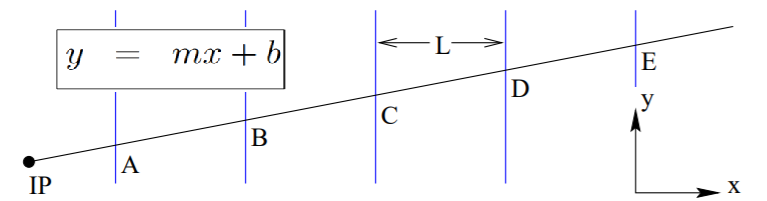
\includegraphics[scale=0.7]{Figures/MEG/Kutschke_Kalman.png}
        \caption[2D kalman linear filter]{Pictorial view of a 2D trajectory of a particle moving along a straight line and interacting with a number of equally spaced tracking stations \cite{Kutschke}. The stations measure the $y$ positions and the goal is to determine the track parameters at some Initial Point (IP). The $x$ origin is positioned on the last station while the $y$ origin is not relevant for this exercise.}
        \label{_Kutschke_Kalman}
    \end{figure}

    \paragraph{Initialization} 
        The first step is to provide a \textit{seed} for the procedure. 
        This is normally done with a pattern recognition algorithm which determines an initial estimate of the parameters, while $V$ is assumed diagonal and with large values.
        \begin{align*}
            \eta = \begin{bmatrix} m_0 \\  b_0 \end{bmatrix},\ \ V=\begin{bmatrix} V_{mm,0}& 0 \\ 0& V_{bb,0} \end{bmatrix}
        \end{align*}

    \paragraph{First hit} 
        The procedure continues by adding point E and is simply necessary to apply the equations \ref{eq_Kalman}, (the explicit calculation can be found in \cite{Kutschke}):

        \begin{gather*}
            V^{(1)}\approx \begin{bmatrix}
            V_{mm,0} & 0 \\ 0 & \sigma^2
            \end{bmatrix}\\
            \eta^{(1)} = 
            \begin{bmatrix} m_0 \\  b_0 \end{bmatrix} +
            \begin{bmatrix} V_{mm,0} & 0 \\ 0 & \sigma^2 \end{bmatrix}
            \begin{bmatrix} 0 \\ 1 \end{bmatrix}
            \frac{y_E-b_0}{\sigma^2}
            = \begin{bmatrix}
            m_0 \\ y_E
            \end{bmatrix}
        \end{gather*}
        It is pretty straightforward to understand that employing just one hit provides information only on the track impact parameter, while there is no information on the trajectory slope.

\paragraph{Transport} 
At this point the track is transported from E to D and, to do this, 
it is helpful to define a new coordinate system located on the second measurement plane. 
In this system the trajectory is $y^\prime=m^\prime x^\prime+b^\prime$ with $y=y^\prime$, $x^\prime=x+L$, $m^\prime=m$ and $b^\prime=b-mL$. 
By defining $A_{i,j}=\frac{\partial \eta_i^\prime}{\partial_j\eta}$,
the same track can represented in a new base:
\begin{gather*}
\eta^{(1^\prime)}=\begin{bmatrix} m_0 \\ y_E - m_0L \end{bmatrix} \\
V^{(1^\prime)} = AV^{(1)} A^T= \begin{bmatrix}
V_{mm,0} & -LV_{mm,0} \\ -LV_{mm,0} & \sigma^2 +L^2V_{mm,0}
\end{bmatrix}
\end{gather*}
As expected, the uncertainty on the slope remains unchanged by this transport, 
while the error on the impact parameter is now increased since the extrapolation used a slope with large uncertainty.

\paragraph{Second hit} 
Since the track is now defined in the coordinate system of the second plane, 
adding the point D and applying again the Kalman equations \ref{eq_Kalman} is straightforward. 
The derivatives take the simple form: $D=\begin{bmatrix}0\\1\end{bmatrix}$. 
we can skip the calculations and simply report the new estimators:

\begin{equation}
\begin{gathered}
V^{(2)}\approx
\begin{bmatrix}
\frac{2\sigma^2}{L^2} & -\frac{\sigma^2}{L} \\
-\frac{\sigma^2}{L} & \sigma^2
\end{bmatrix}\\
\eta^{(2)} = 
\begin{bmatrix} m_0 \\  y_E-m_0L \end{bmatrix} +
V^{(2)}
\begin{bmatrix} 0\\1 \end{bmatrix}
\frac{y_D-(y_E-m_0L)}{\sigma^2} \approx
\begin{bmatrix} \frac{y_E-y_D}{L} \\ y_D\end{bmatrix}
\end{gathered}
\label{eq_V2}
\end{equation}
The interesting feature is that all the assumed starting values have no impact on the estimates: $m_0,\ b_0,\ V_{mm,0}$ and $V_{bb,0}$. 
The uncertainty on the impact parameter is function of solely the local information ($\sigma$), 
while $V_{mm}$ depends on both $\sigma$ and $L$. 

\paragraph{Transport and third hit} 
In order to add a third measurement, 
the same two steps are needed: 
express the same track in the new base and then add the hit. 
The calculations are again detailed in \cite{KutschkePaper} and we will only report the result:
\begin{gather*}
V^{(3)}\approx
\begin{bmatrix}
\frac{\sigma^2}{2L^2} & -\frac{\sigma^2}{2L} \\
-\frac{\sigma^2}{2L} & \frac{5}{6}\sigma^2
\end{bmatrix}\\
\eta^{(3)} \approx
\begin{bmatrix} \frac{y_E-y_C}{2L} \\ \frac{2y_D-y_E+5y_C}{6}
\end{bmatrix}
\end{gather*}
It is interesting to notice that once the third point has been added, 
the diagonal elements of the covariance matrix are reduced with respect to the case with only two points. 

\paragraph{Finishing} Once the procedure has been iterated  to reach point A, 
the estimators of the trajectory use all the available information and are valid in a neighborhood region of A. 
To extrapolate to the track IP, 
the procedure is the same as before, 
describing the trajectory in the coordinate system set in the IP. 

\status{review}
\subsection{Adding multiple scattering}
How does the problem of track fitting change if the detectors are not ideal planes but consist of a thin scattering volume? 
The initialization and the inclusion of the first hit do not change. 
The uncertainty due to multiple scattering on the first hit is negligible because of the starting covariance matrix. 
In this simple model, the scattering is \textit{local} and contributes only to the slope error and not the off-diagonal terms 
and the intercept, but as the track is extrapolated away from the surface it contributes to these terms as well.\\
If the surface introduces a factor $\delta$ in the error of the slope, 
the matrix in eq \ref{eq_V2} the vector remains the same while the matrix becomes
$$
V^{(2)}\approx
\begin{bmatrix}
\frac{2\sigma^2}{L^2}+\delta^2 & -\frac{\sigma^2}{L} \\
-\frac{\sigma^2}{L} & \sigma^2
\end{bmatrix}\\
$$
From this point on the presence of $\delta$ can change substantially the results because at the next iteration, it will enter in both $V^\prime$ and $\eta^\prime$.
 In \cite{KutschkePaper} the calculations are extensively developed up to the third point (point C) 
 with the specific example $\delta^2L^2=\sigma^2$ to keep the passages easy to follow.

\status{review}
\printbibliography[
    title=Bibliography on Kalman filter
]